\documentclass{article}
\title{Diffusion and Score-based Generative Models}
\author{Simone Petruzzi-1811872 Domenico Tersigni-}
\date{August 2023}
\usepackage[margin=1.5in]{geometry} % Adjust the values as per your requirements
\usepackage{amssymb}
\usepackage{amsfonts}
\usepackage{amsmath}
\usepackage{graphicx}
\graphicspath{ {./images/} }

\begin{document}
   \maketitle
   \section{Introduction}
	Given a dataset $\{ x_1,x_2,...,x_n \}$ where each point is drawn independently from an underlying distribution $p(x)$, the goal of generative modelling is to fit a model to the data distribution, such that we can synthetize new data points at will by sampling from the model of the distribution.\newline
	Let's say $p_{data}$ is our model and $x_i$ $\sim$ $p_{data}$. We want to find a single probability distribution, minimizing the distance from $p_{data}$ to $p_{\theta}$. Afterwards we can generate samples from $p_{\theta}$. In order to estimate the model we can use as starting point a Gaussian distribution (basically a computational graph composed by two layers). However a single Gaussian is too simple and we want to leverage on a bigger and deeper computational graph. Thus we want to use deep neural networks to represent complex data distributions. This kind of architectures typically convert high dimensional input into one dimensional output $f_{\theta}(x)$, this output should be converted into a probability density and for this reason we take the exponential of the output in order to make it always positive. Then we normalize by means of a constant $Z_{\theta}$ obtaining:\newline
	\begin{equation}
	p_{\theta}(x) = \frac{e^{f_{\theta}(x)}}{Z_{\theta}}
	\end{equation}
	$Z_{\theta}$ by definition should be computed by evaluating the high dimensional integral of the exponential function of out $\theta$, over all possible values of x in the space:
	\begin{equation}
	Z_{\theta}= \int_{}^{} e^{f_{\theta}(x)} \,dx 
	\end{equation}
	In case of deep neural networks the computation of this integral becomes intractable (NP-complete problem). In order to tackle with the intractability of the normalizing constant, this proposal aims to work with \textbf{score functions}.
	\newpage
   \section{Score-based generative modeling}
	The score funcion is a vector field that gives the direction where the density fucntion grows most quickly. We define the score of a probability density $p(x)$ to be:
	\begin{equation}
	p(x) = \nabla_{x}\ log\ p(x)
	\end{equation}
	Score function is good since in anytime given the density function we can compute the score function very easily by simply texting the dervative. Conversely given the score function we can recover the density function in principle by computing the integral. Thus, we argue that score function mantains preseved all mathematical information of the density function, being computationally more easy to deal with. Indeed with score functions we don't have any normalization restriction:
	\begin{equation}
	\nabla_{x}\ log\ p_{\theta}(x) = \nabla_{x}f_{\theta}(x)\ - \nabla_{x}\log Z_{\theta}
	\end{equation}
	the term $\nabla_{x}\log Z_{\theta}$ is always 0 because it is the gradient of a constant. Thus the score function is the gradient of the deep neural network $f_{\theta}(x)$. We define the score model $s_{\theta}(x)$ as:
	\begin{equation}
	\nabla_{x}f_{\theta}(x) = s_{\theta}(x)
	\end{equation}
	and we want to develop a technique that allows us to train $s_{\theta}(x)$, in order to estimate the underlying score function from a limited set of training data points
	\subsection{Score matching}
	We must train our score model to be close to our ground-truth data score function. Mathematically we can capture the distance between the two vector fields of score by the \textbf{Fisher divergence objective}:
	\begin{equation}
	\frac{1}{2}E_{p_{data}(x)}[||\nabla_{x}\ log\ p_{data}(x) - s_{\theta}(x) ||_{2}^{2}]
	\end{equation}		
	However Fisher divergence can not be computed since we don't know the ground trith value of the data score function $\nabla_{x}\ log\ p_{data}(x)$. There is a way for addressing this challenge and the method is called \textbf{score matching}. Score matching uses integration by parts of Gauss' theorem to convert Fisher divergence into the following equivalent objective:
	\begin{equation}
	E_{p_{data}(x)}[\frac{1}{2}||s_{\theta}(x)||_{2}^{2} + trace(\nabla_{x}\ s_{\theta}(x))]
	\end{equation}
	where $\nabla_{x}\ s_{\theta}(x)$ denotes the Jacobian of $s_{\theta}(x)$. We call it score matching objective, and it is equivalent to the fisher divergence up to a costant. Since constants do not affect optimization, their score matching objective defines the same optimum as the Fisher divergence. In score matching there is no dependency on the score function of the data distribution anymore. Moreover the expectation in score matching can be efficiently be approximated by using empirical mean:
	\begin{equation}
	E_{p_{data}(x)}[\frac{1}{2}||s_{\theta}(x)||_{2}^{2} + trace(\nabla_{x}\ s_{\theta}(x))] \approx \frac{1}{N} \sum_{i=1}^{N}[\frac{1}{2}||s_{\theta}(x)||_{2}^{2} + trace(\nabla_{x}\ s_{\theta}(x_i))]
	\end{equation}
	again this is not scalable to compute since we need one forward propagation to compute the first element of the score function output and we need a backpropagation to compute the first element on the diagonal of its Jacobian. This procedure has to be repeated multiple times until we recovered all diagonal elements on the Jacobian (trace is given by the sum over the diagonal elements). Thus, number of backpropagations needed is proportional to the dimenstionality of our data points. It follows that the whole procedure when modelling high dimensional data like images, requires a lot of backpropagations making this naive score matching approach not scalable.
	\subsection{Sliced score matching}
	This approach aims to solve the problem of naive score matching: the basic intuition is that we want to convert high dimensional problem to a one-dimensional one (since it is much easier to solve). \\
	The idea is to leverage on random projection, this is done in order to approximate $trace(\nabla_{x}\ s_{\theta}(x))$ and get one-dimensional scalar fields. Again to capture this intuition we use sliced Fisher divergence:
	\begin{equation}
	\frac{1}{2}E_{p_{v}}E_{p_{data}(x)}[(\mathbf{v}^{T}\nabla_{x}\ log\ p_{data}(x) - \mathbf{v}^{T}s_{\theta}(x) )^{2}]
	\end{equation}
	also there we apply integration by parts and obtain sliced score matching:
	\begin{equation}
	E_{p_{v}}E_{p_{data}(x)}[\mathbf{v}^{T}\nabla_{x} s_{\theta}(x) \mathbf{v}\ +\frac{1}{2}||s_{\theta}(x)||_{2}^{2}]
	\end{equation}
	$\mathbf{v}^{T}$ $\nabla_{x}s_{\theta}(x)\mathbf{v}$ is much more scalable to compute. It is not hard to find that we can rewrite:
	\begin{equation}
	\mathbf{v}^{T}\nabla_{x}s_{\theta}(x)\mathbf{v} = \mathbf{v}^{T}\nabla_{x}(\mathbf{v}^{T}s_{\theta}(x))
	\end{equation}
	we just need one forward propagation to get the output $s_{\theta}(x)$ and then we can directly compute the inner product between $\mathbf{v}^{T}$ and $s_{\theta}$.\\
	Sliced score matching provides score estimation for the original $unperturbed$ data distribution.
	\subsection{Denoising score matching}
	Another approach is denoising score matching which estimates the scores of $perturbed$ data distribution.\\
	Indeed, the idea here is to perturb the original data distribution employing a perturbation kernel $q_{\sigma}$, then estimate the score function of the noisy data density instead of the original one.
	\begin{equation}
	p_{data}(x)\ \longrightarrow q_{\sigma}(\tilde{x}|x)\ \longrightarrow q_{\sigma}(\tilde{x})
	\end{equation}
	We employ score matching to estimate the score of the perturbed data distribution $q_{\sigma}(\tilde{x})$, and when the perturbation is very small, we can approximately consider the score function of the noisy data density as equivalent to the score function of the noise-free data density. The denoising score matching objective function has been proved equivalent to the following
	\begin{equation}
	\frac{1}{2} \mathbb{E}_{p_{data}(x)} \mathbb{E}_{q_{\sigma}(\tilde{x}|x)}[||s_{\theta}(\tilde{x}) - \nabla_{\tilde{x}}logq_{\sigma}(\tilde{x}|x)||_{2}^{2}]
	\end{equation}
	in this approach we must take care of the trade-off between the quantity of the noise injected. If you want to work well in estimating score functions of noise-free data densities, you need a very small $\sigma$. However when $\sigma$ is too small, the variance of the objective function becomes bigger and eventually explodes. 
   \subsection{Langevin dynamics}
   Now that we have trained our score model to estimate the underlying score function $s_{\theta} \approx \nabla_{x} log p(x)$ we want a method for generating new data points from the given vector field of score functions.\\
   Langevin dynamics is an iterative procedure that allows to draw samples from our score model. The procedure is as follows:
   \begin{itemize}
   	\item Initialize the sample from an arbitrary prior distribution: $x^{o} \sim \pi(x)$, then repeat this for $z^{t} \leftarrow 1,2,...,T\ z^{t} \sim \mathcal{N}(0,I)$
	\item In each sampling step, first generate a random Gaussian vector from the standard Gaussian distribution, then modify x according to the following recurrence:
	\begin{equation}
	x_{t} \leftarrow x^{t-1} + \frac{\epsilon}{2} \nabla_{x} log\ p(x^{t-1})+\sqrt{\epsilon}\ z^{t}
	\end{equation}
   \end{itemize}
   We basically update the previous sample using our score function, plus a scaled version of the Gaussian noise vector. If $\epsilon \rightarrow 0$ and $T \rightarrow \infty$, we are guaranteed to have $x^{t} \sim p(x)$.\\
   It becomes very natural to replace the score function in Langevin dynamics with our score model ($s_{\theta}(x) \approx \nabla_{x}log\ p(x)$), then we can generate new data samples, defining a new generative model.
   \newline
   \subsection{Naive score-based generative modeling and its pitfalls}
   This procedure has drawbacks: we have at first problem in estimating correctly the score function in low data density regions. In those regions we usually don't have enough samples to estimate the score function accurately. Remember that score matching minimizes the expected squared error of the score estimates, $i.e., \frac{1}{2}\mathbb{E}_{p_{data}(x)}[||\nabla_{x}\ log\ p_{data}(x) - s_{\theta}(x) ||_{2}^{2}]$. In practice the expectation is always estimated using i.i.d samples $\{ x_{i}\}_{i=0}^{N} \sim p_{data}(x)$ and when there is a lack of them, the estimation is inaccurate.\\
   \newline
    Also, Langevin dynamics,  when two modes of the data distribution are separated by low density regions, will be not able to recover the relative weights of these two modes in reasonable time. Langevin dynamics can produce correct samples in theory, but it may require a very small step size and  a very large number of step to mix, increasing drastically the computation time.
    \newpage
    \section{Score-based generative modeling with multiple noise perturbations}
    In the previous section we talked about score-based generative modeling and it's problems. The main problem of that approach is bad estimation of the score function in low data density regions. We can address this challenge by injecting Gaussian noise to perturb our data data points and then doing the exact same procedure on the perturbed data. After having added enough Gaussian noise we provide useful directional information for Langevin dynamics, also score functions of noisy data densities are much easier to be estimated accurately. \\
    \newline
    However by simply injecting Gaussian noise we don't solve the problem, because after perturbing data points, the noisy data densities distances, are no longer good approximation for the original data density. How to choose the right level of noise ? To solve this, we can use multiple noise levels simultaneously and consider a noise conditional score model. This model takes noise level $\sigma$ as additional input dimension to the model and the output corresponds to the score function of the perturbed data density by $\sigma$.  We perturb the data distribution $p(x)$ with a Gaussian noise $\mathcal{N}(0,\sigma_{i}^{2}I), i=1,2,...,L$, obtaining the noise-perturbed distribution:
    \begin{equation}
    p_{\sigma_{i}}(x) = \int p(y)\ \mathcal{N}(x;y,\sigma_{i}^{2}I) dy
    \end{equation}
    We choose $\sigma_{1}$ large enough such that we don't have problems in low density regions, and $\sigma_{L}$ small enough to minimize the effect on data.\\
    Built upon this intuition we improve score-based generative modeling by first perturbing data as written above, then simultaneously estimate scores corresponding to all noise levels by training a single noise conditional core network.
    \subsection{Noise conditional score network}
    We aim to train this network to jointly estimate the scores of all perturbed data distributions, $i.e., \forall \sigma \in \{ \sigma_{i} \}_{i=1}^{L}$ : $s_{\theta}(x,\sigma) \approx \nabla_{x}logq_{\sigma}(x)$. We call $s{\theta}(x,\sigma)$ a $Noise\ Conditional\ Score\ Network$ (NCSN).
    \subsection{NCSN learning with score matching}
    Again for training this kind of network we can leverage on score matching techniques (both sliced and denoising score matching). Here we adopt denoising score matching loss function:
    \begin{equation}
    \frac{1}{2N} \sum_{i=1}^{N} \lambda(\sigma_{i})\ \mathbb{E}_{p_{\sigma_{i}}}(x) [ || \nabla_{x}\ log {p_{\sigma_{i}}} (x) - s_{\theta}(x,\sigma_{i}) ||_{2}^{2}]
     \end{equation}
     and in the special case of Gaussian perturbations, we can simplify the denoising objective as:
     \begin{equation}
      \frac{1}{2N} \sum_{i=1}^{N} \lambda(\sigma_{i})\ \mathbb{E}_{p_{\sigma_{i}}}(x)[|| s_{\theta}(\tilde{x},\sigma)+ \frac{\tilde{x}-x}{\sigma^{2}}||_{2}^{2}]
     \end{equation}
     $\lambda(\sigma_{i})$ is a positive weighting function (often chosen to be $ \lambda(\sigma_{i}) = \sigma_{i}^{2} $), which balances the scales of score matching across all noise levels, making helpful for optimization.
     \subsection{NCSN sampling with annealed Langevin dynamics}
     Given the trained noise conditional score model we can use annealed Langevin dynamics to produce samples. We start this process by initializing the samples from some fixed prior distribution, then we first apply Langevin dynamics to sample from the score model with the biggest perturbation noise, let's say $q_{\sigma_{1}}(x)$. Next we run Langevin dynamics to sample from $q_{\sigma_{2}}(x)$, starting from the final samples of the previous simulation. This procedure continues until eventually we reach the score function with the smallest noise level, running Langevin dynamics to sample from $q_{\sigma_{L}}(x)$, which is close to $p_{data}(x)$ when $\sigma_{L} \approx 0$.\\
     \newline
     When $\sigma_{1}$ is sufficiently large, the low density regions of $q_{\sigma_{1}}(x)$ become small and the modes become less isolated. Also as discussed previously the score estimation is more accurate. We can argue that Langevin dynamics produces good samples for $q_{\sigma_{1}}(x)$, and also that those samples are likely to come from high density regions of $q_{\sigma_{1}}(x)$, meaning that this is valid also for $q_{\sigma_{2}}(x)$ (given that $q_{\sigma_{1}}(x)$ and $q_{\sigma_{2}}(x)$ slightly differ each other), and so on. Thus as score estimation and Langevin dynamics perform better in high density regions, samples from $q_{\sigma_{i-1}}(x)$ provide good initial point for $q_{\sigma_{i}}(x)$. Finally we obtain good samples of good quality from $q_{\sigma_{L}}(x)$ that is our last step.
     \newpage
     \section{Score-based generative modeling with stochastic differential equations}
     As already discussed, adding multiple noise scale is critical for the success of score-based generative models. In this section the aim is to generalize the previous framework (that is using a finite number of noise levels), to use an infinite number of noise levels. By generalizing the number of noise scales to infinity, we obtain not only high quality samples, but also, among others, exact log-likelihood computation, and controllable generation. Specifically we consider a continuum of distribution that evolve over time according to a diffusion process that progressively diffuses a data point itno random noise, and is given by a SDE (Stochastic Differential Equation) that does not depend on the data and has no trainable parameters. After the training procedure, by reversing the previous process, we can mold random noise into data for sample generation. This reverse process relys on a reverse-time SDE, which can be derived from the forward SDE given the score of the marginal probbility densities as function of time. Therefore we can approximate the reverse-time SDE with a time-dependent neural network which estimates the scores, and then produce samples by simply using numerical SDE solvers.\\
      \begin{figure}[h]
	  	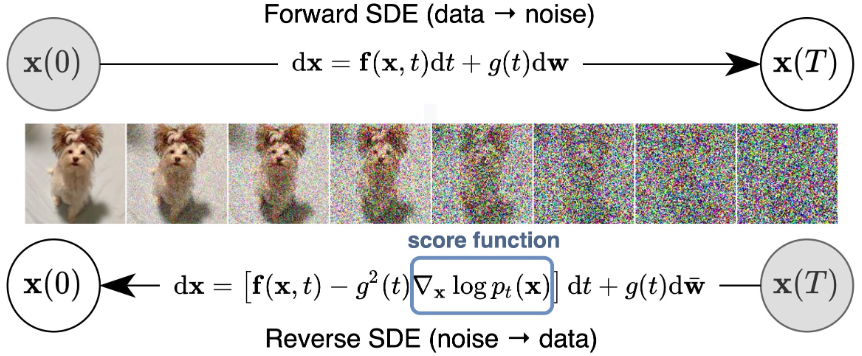
\includegraphics[width=11cm]{SDEmodel}
	  	\centering
	  \end{figure}
	\subsection{Perturbing data with SDEs}
When the number of noise scales approaches infinity, we essentially perturb the data distribution with continuously growing levels of noise. The perturbation procedure is a continuous time stochastic process. Our goal is to construct a diffusion process that is solution of a stochastic differential equation. This diffusion process $\{ x(t) \}_{t=0}^{T}$ can be modeled as the solution of the following SDE:
	\begin{equation}
	 dx= f(x,t)dt + g(t)dw
	\end{equation}
	where $f(.,t): \mathbb{R}^{d} \rightarrow \mathbb{R}^{d}$ is a vector-valued function called drift coefficient of $x(t)$ (controls deterministic properties of the stochastic process), $g(.): \mathbb{R} \rightarrow \mathbb{R}$ is a scalar function known as the diffusion coefficient of $x(t)$, and w is the standard Wiener process. The $dw_{t}$ can be seen as the infinitesimal Gaussian noise the each time is injected.\\
	The solution of a stochastic differential is continuous collection of random variables that trace stochastic trajectories as the time grows. Let $p_{t}(x)$ denote the marginal probability density function of $x(t)$ with $t \in [0,T] $, clearly $p_{0}(x)$ is the data distribution with no perturbation. After perturbing the data distribution with enough noise , $p_{T}(x)$ becomes close to a tractable noise distribution $\pi (x)$ that is called prior distribution. \\
	\newline
	A specific differential equation that we can use for this purpose (choice of SDE isn't unique) could be:
	\begin{equation}
	dx=e^t\ dw
	\end{equation}
	it perturbs data with a Gaussian noise of mean zero and exponentially growing variance
	\subsection{Reversing the SDE for sample generation}
For a finite number of noise scales, we can generate samples by reversing the perturbation process using annealed Langevin dynamics, i.e, sequentially sampling from each noise perturbed distribution using Langevin dynamics. For infinite noise scales we can do the same as the Langevin dynamics by reversing the forward SDE. Thus by starting form samples of $x(T) \sim p_{T}$ and reversing the process, we can obtain samples $x(0) \sim p_{0}$. It was proved that the reverse of a diffusion process is also a diffusion process, and any SDE has corresponding reverse SDE. The reverse SDE in our case is:
	\begin{equation}
	dx = [f(x,t)-g(t)^2 \nabla_{x}logp_{t}(x)]dt+g(t)d \bar{w}
	\end{equation}
	where $\bar{w}$ is a standard Wiener process when the time flows backwards from T to 0, and $dt$ is the infinitesimal reverse (negative) time step. In order to estimate the reverse SDE we must compute $\nabla_{x}logp_{t}(x)$, which is exactly the score function of $p_t(x)$
     \subsection{Estimating the reverse SDE with score-based models and score matching}
     In order to solve the reverse SDE is required the terminal distribution $p_{T}(x)$ and the score function $\nabla_{x}logp_{t}(x)$. To estimate the score function we can train a time-dependent score-based model $s_{\theta}(x,t)$. The objective function is a continuous weighted combination of Fisher divergence:
     \begin{equation}
	 \theta^*= \mathop{argmin}_{\theta} \mathbb{E}_{t} \{ \lambda(t) \mathbb{E}_{x(0)} \mathbb{E}_{x(t)|x(0)} [||s_{\theta}(x(t),t) - \nabla_{x}logp_{0t}(x(t)|x(0))||_{2}^{2}] \} 
	 \end{equation}      
	 Here $\lambda$ : $[0,T] \rightarrow \mathbb{R}_{>0}$ is a positive weighting function and $x(0) \sim p_{0}(x)$ and $x(t) \sim p_{0t}(x(t)|x(0))$. As before, this combination of Fisher divergence can be optimized efficiently with score metching methods and once the model is trained we can plug it into the reverse SDE.\\
	 When $\lambda(t) = g^2(t)$, we have an important connection between the combination of Fisher divergence and the Kullback-Leibler divergence form $p_{0}$ to $p_{\theta}$ under some regularity conditions. Since the KL divergence is directly related to maximal likelihood training, by minimizing the score function with this particular likelihood of weighting functions, we  are implicitly maximizing likelihoods.
	 \begin{equation}
	 KL(p_{0}(x) || p_{\theta} \leq \frac{1}{2} \mathbb{E}_{t \sim Uniform [0,T]}[\lambda || \nabla_{x}logp_{t}(x)-s_{\theta}(x,t)||_{2}^{2}] + KL(p_{t} || \pi)
	 \end{equation}
	 $KL(p_{t} || \pi) \approx 0$ if T is large enough and this does not affect the optimization procedure, since it does not depend on model parameter $\theta$.
	 \subsection{Solving the reverse SDE}
	 After having trained a time-depedent score model $s_{\theta}$, we can use it to construct the reverse-time SDE and generate samples. We can basically use any numerical stohastic differential equation solver: a simple approach is Euler-Maruyama, which is a stochastic generalization to the classical Euler solver fo ordinary differential equations. When applied to our estimated reverse SDE, it discretizes the SDE using finite time steps and small Gaussian noise: specifically, it chooses a small negative step $\Delta t \approx 0$, initializes $t \leftarrow T$, then iterates the following procedure until $t \approx 0$:
	 \begin{equation} \begin{split}
	 &\Delta x \leftarrow [f(x,t) - g^2(t)s_{\theta}(x,t)] \Delta t + g(t) \sqrt{|\Delta t|}z_{t} \\
	 &x \leftarrow x+ \Delta x \\
	 &t \leftarrow t+ \Delta t
	 \end{split} \end{equation}
	 where $z \sim \mathcal{N}(0, |\Delta t| I)$.
	 Aside the Euler-Maruyama method, other numerical SDE solver can be used.\\
	 \newline
	 Since we have additional information that can be used, we can improve simple generic SDE solvers. Since we have a score-based model $s_{\theta}(x,t) \approx \nabla_{x} log\ p_{t}(x)$, and we only care about sampling for each marginal distribution $p_{t}(x)$, we can employ score-based MCMC (Markov Chain Monte Carlo) approaches such Langevin MCMC (Parisi, 1981) to fine-tune the trajectories obtained by the solver. Specifically we can use a predictor-corrector method. At each time step, the numerical SDE solver first gives an estimate of the sample at next time step (playing role of "predictor"). Then, the score based MCMC approach corrects the marginal distribution of estimated sample (playing the role of "corrector")
	 \subsection{Probability flow and connection to neural ODEs}
	 With this kind of continuous SDE approach, we do not only improve the empirical performace (sample generation), but also we can accurately compute the exact log-likelihood. This requires to convert the stochastic differential equation into an ordinary one without changing its marginal distributions $\{p_{t}(x)\}_{t \in [0,T]}$. Thus by solving this ODE, we can sample from the same distributions as the reverse SDE. The corresponding ODE of an SDE is named probability flow ODE, given by:
	 \begin{equation}
	 dx=[f(x,t) - \frac{1}{2} g^2(t \nabla_{x}log\ p_{t}(x))]dt
	 \end{equation}
Again this relys only on the score function and we can plug our conditional score model into the ODE in order to solve it. When we plug out conditional score model into the probability flow ODE, it becomes a special case of neural ODE. As such, the probability flow ODE inherits all properties of neural ODEs or continuous normalizing flows, including exact log-likelihood computation. Specifically, we can leverage the instantaneous change-of-variable formula o compute the unknown data density $p_{0}$ from the known prior density $p_{T}$ with numerical ODE solvers.
\end{document}